\documentclass[]{IEEEtran}
% some very useful LaTeX packages include:
%\usepackage{cite}      
\usepackage{graphicx}   
\usepackage{subfigure} 
\usepackage{url}       
\usepackage{amsmath}    
\usepackage{caption2}
% Your document starts here!
\begin{document}

% Define document title and author
	\title{Weekly Report}
	\author{Adviser: Prof. Yang Wen \\Student: Cheng Wensheng\\ Period: 2018.8.5-8.12
	}
	\markboth{Visual Information Processing Group}{}
	\maketitle

% Write abstract here
\begin{abstract}
	This week I mainly put my effort on using traditional methods to extract buildings in SAR images. 
\end{abstract}

% Each section begins with a \section{title} command
\section{Sar contest}
	% \PARstart{}{} creates a tall first letter for this first paragraph
	\PARstart{I}{n} this contest, we only have 10 training images with the size of 1500*1500. At first, we tried RefineNet, and we got the F1 score of 0.57. So this week we tried traditional methods to see the result. And the traditional methods got 0.61 accuracy on the 10 images, but only got 0.51 accuracy on the test set.	
	\begin{itemize}
		\item At first, we use Gaussian filter to remove some noise and make images smoother.  
		\item Then we adopt Otsu's method to binarize the gray image, and get the binarization image. With the binarization image, we apply dilation, erosion, open, close, etc., to refine the boundary. 
		\item  After that, we get all contours of the binarization image, except very small ones, which we consider as non-building. To get the full building, we use rectangle to bound these contours.
		\item  At last, we fill these rectangles with white pixels and consider them as buildings.
	\end{itemize}
	
	Fig.~\ref{fig:fw} is the traditional methods result. Fig.~\ref{fig:rt} is the ground truth image.
	

% Main Part

\newpage
\begin{figure}[!hbt]
%		 Center the figure.
		\vspace{0.7cm}
%		\hspace{50cm}
		\begin{center}
			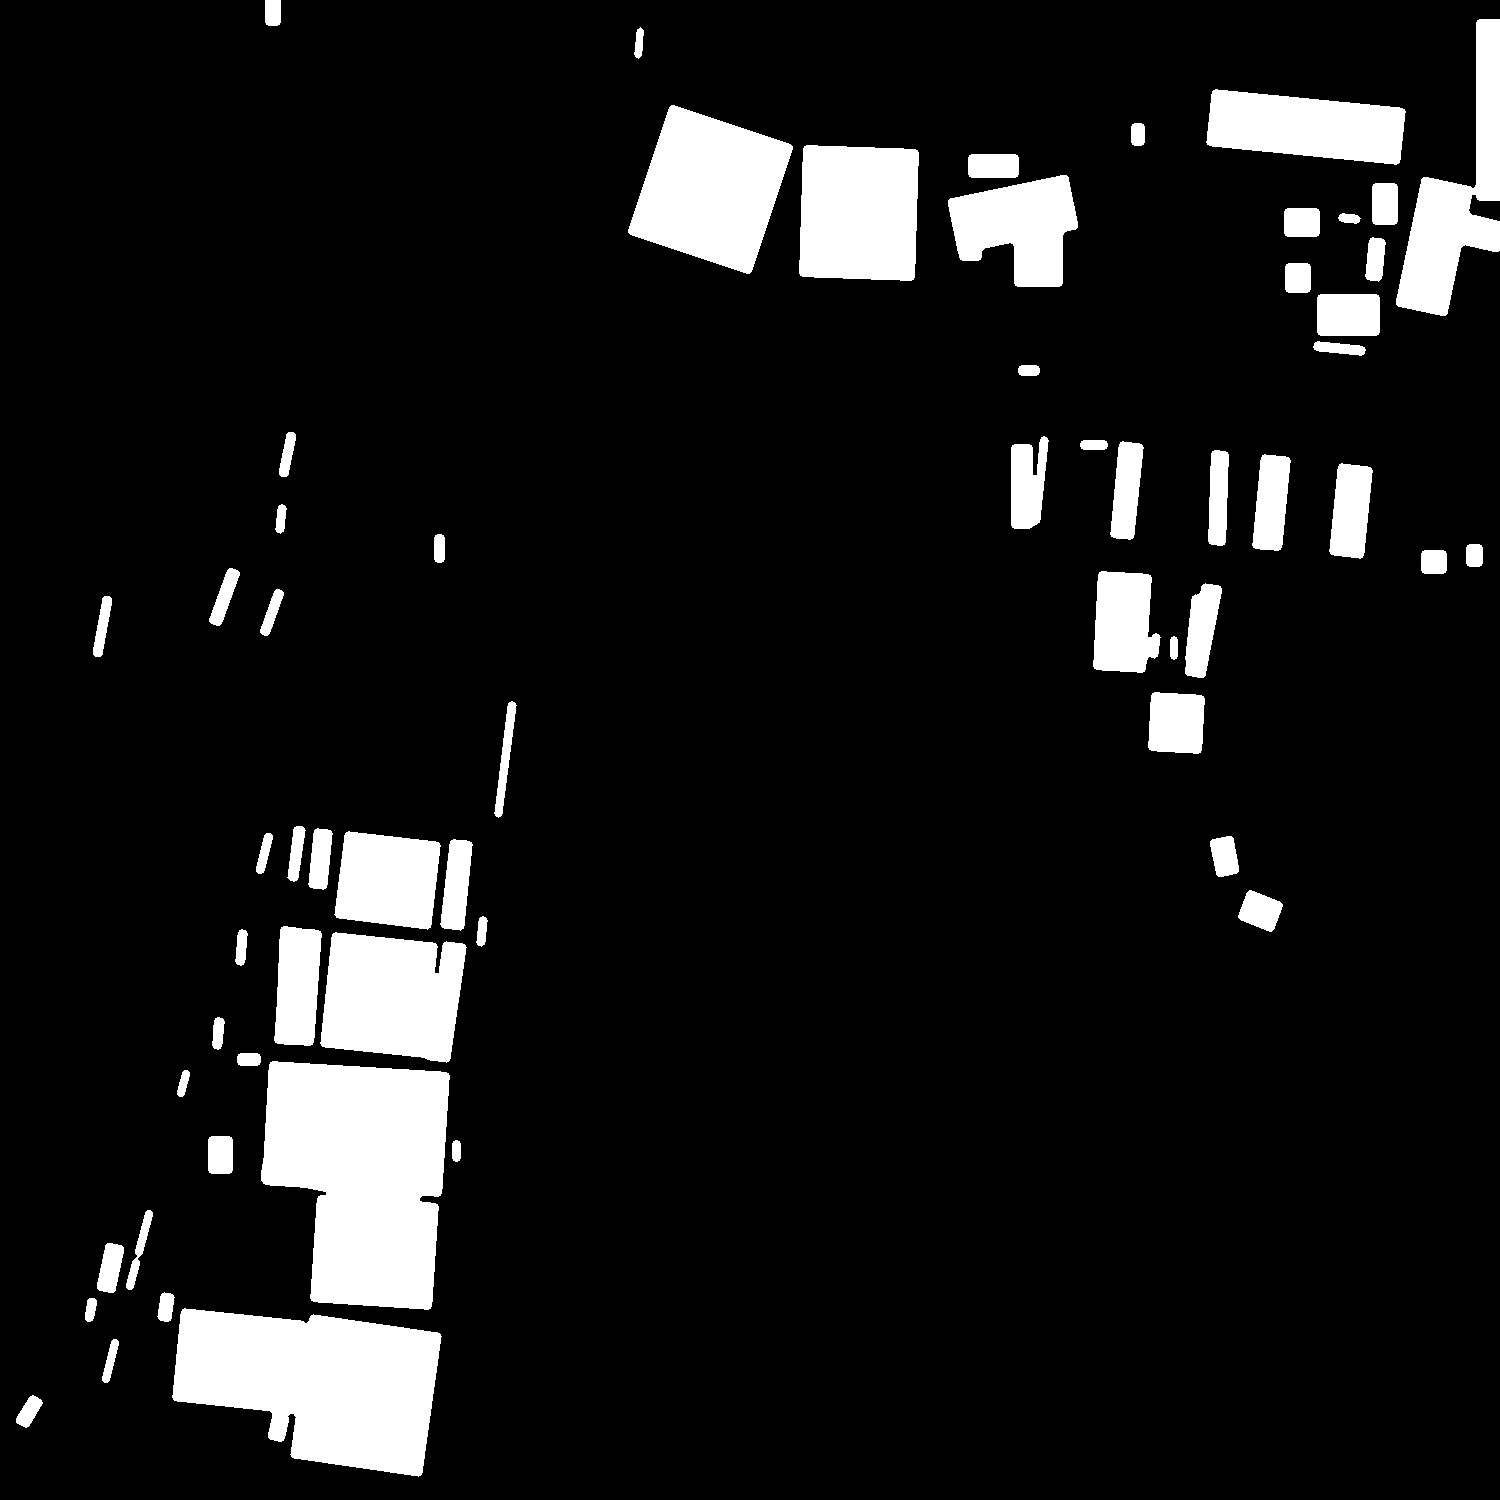
\includegraphics[width=0.7\columnwidth]{fw}
				%		 Create a subtitle for the figure.
			\caption{Traditional methods result}
			\label{fig:fw}
		    \vspace{0.2cm}
			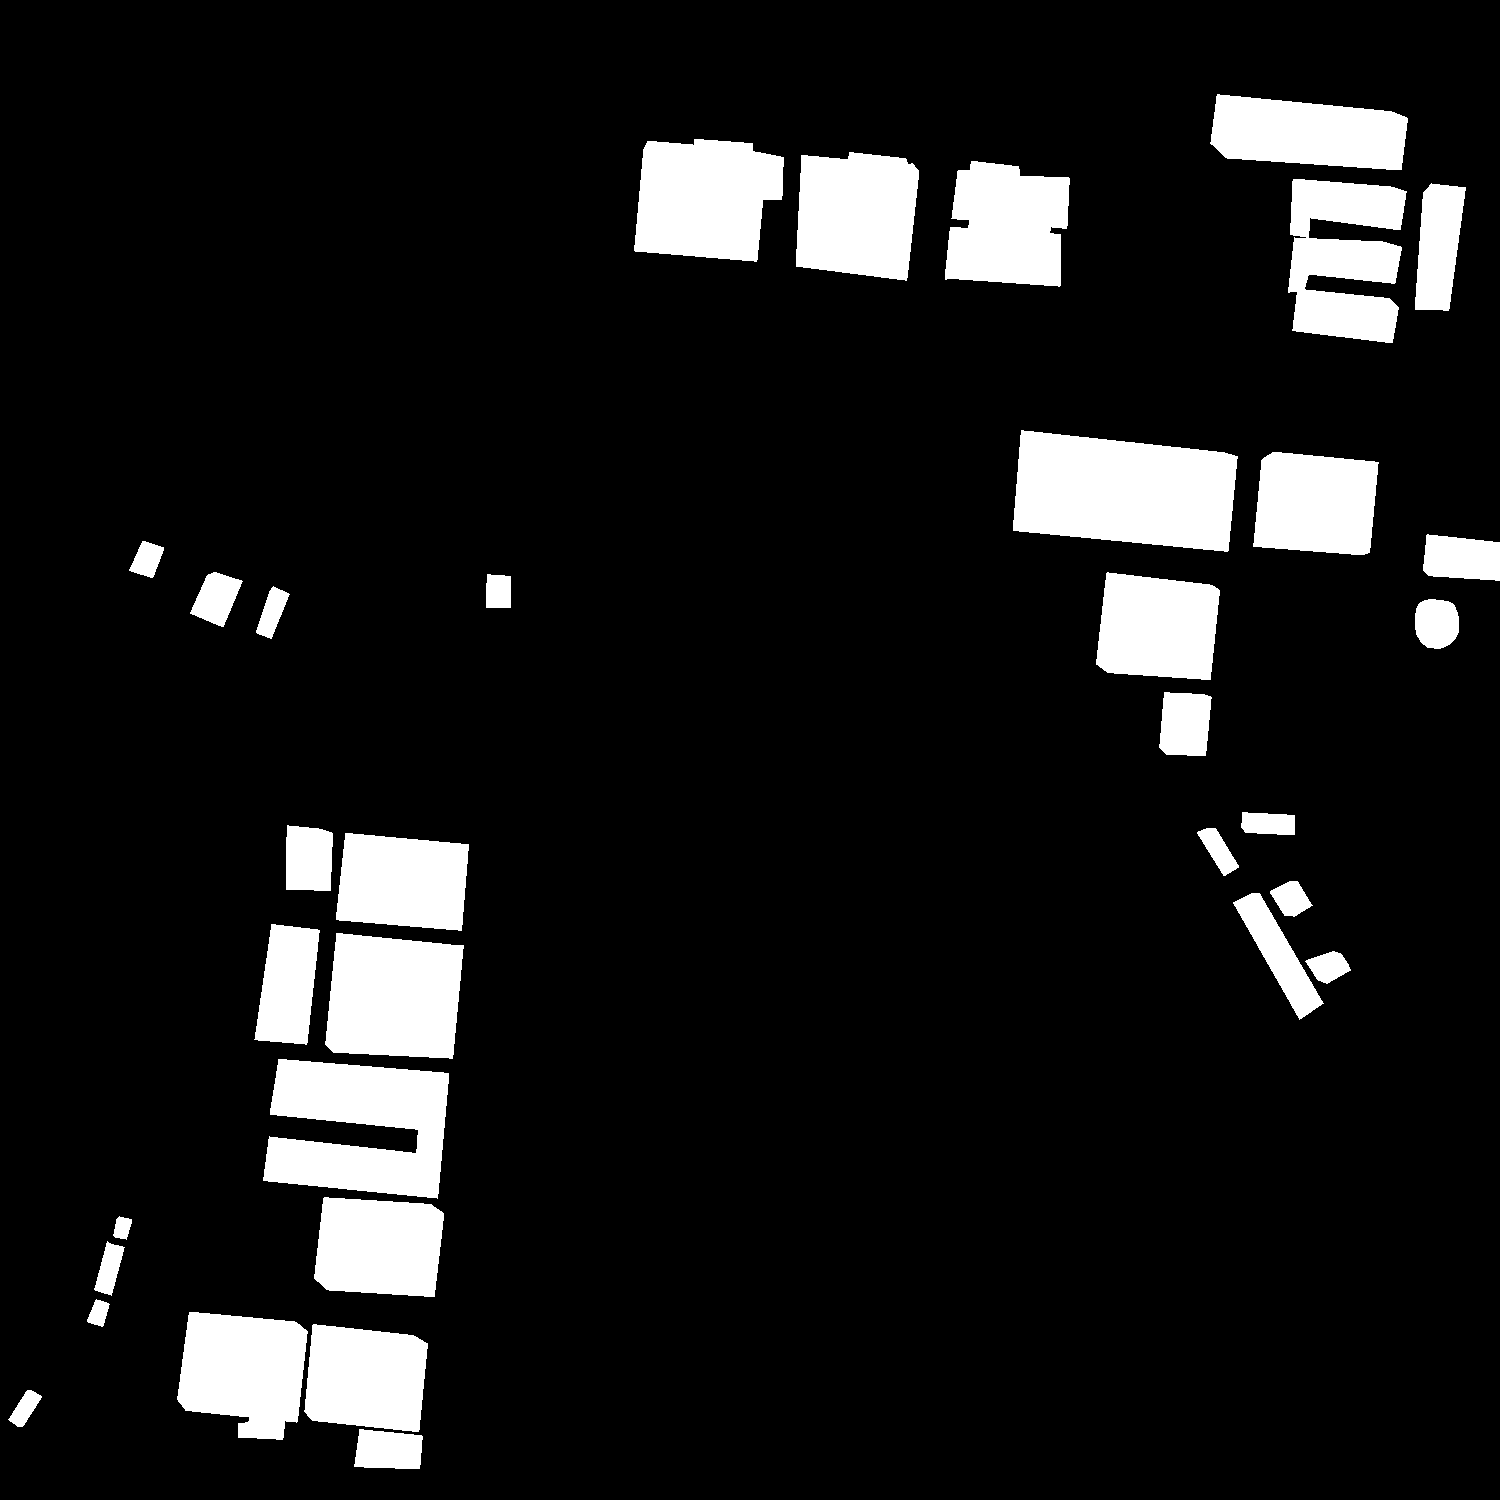
\includegraphics[width=0.7\columnwidth]{rs}
				%Create a subtitle for the figure.
			\caption{Ground truth}
			\label{fig:rt}
		\end{center}
	\end{figure}

% Now we need a bibliography:
%\begin{thebibliography}{5}
%
%	%Each item starts with a \bibitem{reference} command and the details thereafter.
%	\bibitem{HOP96} % Transaction paper
%	J.~Hagenauer, E.~Offer, and L.~Papke. Iterative decoding of binary block
%	and convolutional codes. {\em IEEE Trans. Inform. Theory},
%	vol.~42, no.~2, pp.~429–-445, Mar. 1996.
%
%	\bibitem{MJH06} % Conference paper
%	T.~Mayer, H.~Jenkac, and J.~Hagenauer. Turbo base-station cooperation for intercell interference cancellation. {\em IEEE Int. Conf. Commun. (ICC)}, Istanbul, Turkey, pp.~356--361, June 2006.
%
%	\bibitem{Proakis} % Book
%	J.~G.~Proakis. {\em Digital Communications}. McGraw-Hill Book Co.,
%	New York, USA, 3rd edition, 1995.
%
%	\bibitem{talk} % Web document
%	F.~R.~Kschischang. Giving a talk: Guidelines for the Preparation and Presentation of Technical Seminars.
%	\url{http://www.comm.toronto.edu/frank/guide/guide.pdf}.
%
%	\bibitem{5}
%	IEEE Transactions \LaTeX and Microsoft Word Style Files.
%	\url{http://www.ieee.org/web/publications/authors/transjnl/index.html}
%
%\end{thebibliography}

% Your document ends here!
\end{document}